%%%%%%%%%%%%%%%%%%%%%%%%%%%%%%%%%%%%%%%%%%%%%%%%%%%%%%%%%%%%%%%%%%%%%%%%%%%%%%%%
%%%%%%%%%%%%%%%%%%%%  Set document class, and configure it  %%%%%%%%%%%%%%%%%%%%
%%%%%%%%%%%%%%%%%%%%%%%%%%%%%%%%%%%%%%%%%%%%%%%%%%%%%%%%%%%%%%%%%%%%%%%%%%%%%%%%


% Define the document class
\documentclass[a4paper,nomoderntitles]{tufte-handout}

% Used for adding images/graphics to the document
\usepackage{graphicx}
  % Set default scaling for included graphics
  \setkeys{Gin}{width=\linewidth,totalheight=\textheight,keepaspectratio}
  % Define base path for graphics, change this as needed
  \graphicspath{{graphics/}}

% Improves the quality of tables in LaTeX
% It provides useful commands, and ads some behind the scenes optimizations
% Tables created by this package are similar to the tables in Tufte's books
\usepackage{booktabs}

% Provides a way to set units in typographically correct way
% It includes the `nicefrac' package to provide nicer looking fractions
% Common commands include \unit[<value>]{<unit>}, \nicefrac{<num>}{<den>},
% and \unitfrac[<value>]{<num>}{<den>}
% The \nicefrac can take a font command as an optional argument
\usepackage{units}

% Extends verbatim with new environments, and more features
\usepackage{fancyvrb}
  % Sets default verbatim font, smaller than default
  \fvset{fontsize=\small}

% Changes how the date is displayed in the document,
% and provides extra date related commands
% I prefer the ISO format yyyy-mm-dd, but it can be changed as needed
% Also used to print <month> <year> in the copyright page
\usepackage[style=iso,en-US]{datetime2}

% Can enable or disable hyphenation of words, even in TT font environments
\usepackage[htt]{hyphenat}


%%%%%%%%%%%%%%%%%%%%%%%%%%%%%%%%%%%%%%%%%%%%%%%%%%%%%%%%%%%%%%%%%%%%%%%%%%%%%%%%
%%%%%%  These can be removed in actual documents, only used for examples  %%%%%%
%%%%%%%%%%%%%%%%%%%%%%%%%%%%%%%%%%%%%%%%%%%%%%%%%%%%%%%%%%%%%%%%%%%%%%%%%%%%%%%%


% This package allows for easy insertion of dummy text
\usepackage[language=english]{lipsum}

% Tries to intuit whether or not to add a space after a command
% Used in some documentation commands here, but can be used in other places as well
\usepackage{xspace}

% This package lets writer include fancy TeX logos in text
\usepackage{hologo}

% Used to print LaTeX commands with normalized font styles and environments
% command name, adds backslash automatically
\newcommand{\doccmd}[1]{\texttt{\textbackslash#1}}
% optional command argument
\newcommand{\docopt}[1]{\ensuremath{\langle}\textrm{\textit{#1}}\ensuremath{\rangle}}
% required command argument
\newcommand{\docarg}[1]{\textrm{\textit{#1}}}
% environment name
\newcommand{\docenv}[1]{\textrm{\textbf{#1}}}
% package name
\newcommand{\docpkg}[1]{\texttt{#1}}
% document class name
\newcommand{\doccls}[1]{\texttt{#1}}
% document class option name
\newcommand{\docclsopt}[1]{\texttt{#1}}
% command specification environment
\newenvironment{docspec}{\begin{quote}\noindent}{\end{quote}}

% Shortcut for printing Tufte LaTeX class name
\newcommand{\TL}{Tufte-\hologo{LaTeX}\xspace}


%%%%%%%%%%%%%%%%%%%%%%%%%%%%%%%%%%%%%%%%%%%%%%%%%%%%%%%%%%%%%%%%%%%%%%%%%%%%%%%%
%%  Define document metadata, and other useful things like bibliography file  %%
%%%%%%%%%%%%%%%%%%%%%%%%%%%%%%%%%%%%%%%%%%%%%%%%%%%%%%%%%%%%%%%%%%%%%%%%%%%%%%%%


\title{An Example of the Tufte-Handout Style\thanks{Inspired by Edward Tufte!}}
\author[The Tufte-LaTeX Developers]{The Tufte-\LaTeX\ Developers}
%\date{2025-01-28} % If the \date command is omitted, current date will be used

% Debugging
%\geometry{showframe} % display margins for debugging page layout

% Define BibLaTeX resource file
\addbibresource{sample-bibliography.bib}


%%%%%%%%%%%%%%%%%%%%%%%%%%%%%%%%%%%%%%%%%%%%%%%%%%%%%%%%%%%%%%%%%%%%%%%%%%%%%%%%
%%%%%%%  Main handout contents follow from here, add your document here  %%%%%%%
%%%%%%%%%%%%%%%%%%%%%%%%%%%%%%%%%%%%%%%%%%%%%%%%%%%%%%%%%%%%%%%%%%%%%%%%%%%%%%%%


\begin{document}

% Print title with author and date
\maketitle

% Add an abstract
\begin{abstract}
  \noindent
  This document describes the Tufte handout \LaTeX\ document style.
  It also provides examples and comments on the style's use.
  Only a brief overview is presented here;
  for a complete reference, see the sample book.
\end{abstract}

% Start the main matter (normal sections)
%\section{New Features}
\begin{multicols}{2} [
  %\subsection{Color Showcase}
    The Tufte-\LaTeX\ document classes defines a number of colors.
    It uses these colors for links, citations, sections, and other elements.
    The \docpkg{xcolor} package defines the colors.
    Users can use these colors in their own documents, or redefine them.
    Here are the colors available in the Tufte-\LaTeX\ document classes:
]
\noindent
\fcolorbox{tufte-black}{tufte-black}{\parbox[c][1.0ex][b]{4em}{\phantom{space}}}
\Verb|tufte-black| \\
\fcolorbox{tufte-red}{tufte-red}{\parbox[c][1.0ex][b]{4em}{\phantom{space}}}
\Verb|tufte-red| \\
\fcolorbox{tufte-orange}{tufte-orange}{\parbox[c][1.0ex][b]{4em}{\phantom{space}}}
\Verb|tufte-orange| \\
\fcolorbox{tufte-yellow}{tufte-yellow}{\parbox[c][1.0ex][b]{4em}{\phantom{space}}}
\Verb|tufte-yellow| \\
\fcolorbox{tufte-green}{tufte-green}{\parbox[c][1.0ex][b]{4em}{\phantom{space}}}
\Verb|tufte-green| \\
\fcolorbox{tufte-blue}{tufte-blue}{\parbox[c][1.0ex][b]{4em}{\phantom{space}}}
\Verb|tufte-blue| \\
\fcolorbox{tufte-purple}{tufte-purple}{\parbox[c][1.0ex][b]{4em}{\phantom{space}}}
\Verb|tufte-purple| \\
\fcolorbox{tufte-grey}{tufte-grey}{\parbox[c][1.0ex][b]{4em}{\phantom{space}}}
\Verb|tufte-grey| \\
\fcolorbox{tufte-pastel-red}{tufte-pastel-red}{\parbox[c][1.0ex][b]{4em}{\phantom{space}}}
\Verb|tufte-pastel-red| \\
\fcolorbox{tufte-pastel-orange}{tufte-pastel-orange}{\parbox[c][1.0ex][b]{4em}{\phantom{space}}}
\Verb|tufte-pastel-orange| \\
\fcolorbox{tufte-pastel-yellow}{tufte-pastel-yellow}{\parbox[c][1.0ex][b]{4em}{\phantom{space}}}
\Verb|tufte-pastel-yellow| \\
\fcolorbox{tufte-pastel-green}{tufte-pastel-green}{\parbox[c][1.0ex][b]{4em}{\phantom{space}}}
\Verb|tufte-pastel-green| \\
\fcolorbox{tufte-pastel-blue}{tufte-pastel-blue}{\parbox[c][1.0ex][b]{4em}{\phantom{space}}}
\Verb|tufte-pastel-blue| \\
\fcolorbox{tufte-pastel-purple}{tufte-pastel-purple}{\parbox[c][1.0ex][b]{4em}{\phantom{space}}}
\Verb|tufte-pastel-purple|
\end{multicols}

%\subsection{Note Environments}

Tufte-\LaTeX\ provides two environments for notes. The \docenv{ShadedNote}
environment provides a shaded background. The \docenv{FramedNote} environment
places a frame to the left of the note. Both environments use the same 
counter as they are similar and it doesn't make sense to separate them.

\begin{ShadedNote}
  This is an example of the \Verb|ShadedNote| environment. It provides a
  shaded background for the note text. The note text can be long or short.
\end{ShadedNote}

\begin{FramedNote}[
  name={Note Title},
  label={fn:label}
  ]
  This is an example of the \Verb|FramedNote| environment. It provides a
  framed box to the left of the note text. The note text can be long or short.
\end{FramedNote}

If you label an note, you can reference it using the \doccmd{cref} command.
For example, \cref{fn:label} showcases the \docenv{FramedNote} environment.
You can also use the \docopt{continues} option to continue an note:

\begin{FramedNote}[continues={fn:label}]
  This is a continuation of the previous note. It will be displayed in a new
  frame, but will have the same label, title, and number.
\end{FramedNote}


To use them in your own documents, you need to define the environments using:

\begin{Verbatim}
  \begin{ShadedNote}[
    title={Optional title}, 
    label={Optional label},
    continues={Optional label}
    ]
    Note text here
  \end{ShadedNote}  
\end{Verbatim}

\section{Section Example}
\subsection{Subsection Example}
\paragraph{Paragraph Example}

\section{\TL\ Design}
The Tufte-\LaTeX\ document classes define a style similar to the
style Edward Tufte uses in his books and handouts. Tufte's style is known
for its extensive use of sidenotes, tight integration of graphics with
text, and well-set typography. This document aims to be at once a
demonstration of the features of the Tufte-\LaTeX\ document classes
and a style guide to their use.

\section{Page Layout}\label{sec:page-layout}
\subsection{Headings}\label{sec:headings}
This style provides \textsc{a}- and \textsc{b}-heads (that is,
\Verb|\section| and \Verb|\subsection|), demonstrated above.

The Tufte-\LaTeX\ classes will emit an error if you try to use
\linebreak\Verb|\subsubsection| and smaller headings.

% let's start a new thought -- a new section
\newthought{In his later books},\cite{Tufte2006} Tufte
starts each section with a bit of vertical space, a non-indented paragraph,
and sets the first few words of the sentence in \textsc{small caps}. To
accomplish this using this style, use the \Verb|\newthought| command:  
\begin{docspec}
  \doccmd{newthought\{In his later books\}, Tufte starts\ldots}
\end{docspec}

\subsection{Sidenotes}\label{sec:sidenotes}
One of the most prominent and distinctive features of this style is the
extensive use of sidenotes. There is a wide margin to provide ample room
for sidenotes and small figures. Any \Verb|\footnote|s will automatically
be converted to sidenotes.\footnote{This is a sidenote that was entered
using the \texttt{\textbackslash footnote} command.} If you'd like to place 
ancillary information in the margin without the sidenote mark (the superscript
number), you can use the \Verb|\marginnote| command.\marginnote{This is a
margin note. Notice that there isn't a number preceding the note, and
there is no number in the main text where this note was written.}

The specification of the \Verb|\sidenote| command is:
\begin{docspec}
  \doccmd{sidenote[\docopt{number}][\docopt{offset}]\{\docarg{Sidenote text.}\}}
\end{docspec}

Both the \docopt{number} and \docopt{offset} arguments are optional. If you
provide a \docopt{number} argument, then that number will be used as the
sidenote number. It will change of the number of the current sidenote only and
will not affect the numbering sequence of subsequent sidenotes.

Sometimes a sidenote may run over the top of other text or graphics in the
margin space. If this happens, you can adjust the vertical position of the
sidenote by providing a dimension in the \docopt{offset} argument. Some
examples of valid dimensions are:
\begin{docspec}
  \ttfamily 1.0in \qquad 2.54cm \qquad 254mm \qquad 6\Verb|\baselineskip|
\end{docspec}
If the dimension is positive it will push the sidenote down the page; if the
dimension is negative, it will move the sidenote up the page.

While both the \docopt{number} and \docopt{offset} arguments are optional, they
must be provided in order. To adjust the vertical position of the sidenote
while leaving the sidenote number alone, use the following syntax:
\begin{docspec}
  \doccmd{sidenote[][\docopt{offset}]\{\docarg{Sidenote text.}\}}
\end{docspec}
The empty brackets tell the \Verb|\sidenote| command to use the default
sidenote number.

If you \emph{only} want to change the sidenote number, however, you may
completely omit the \docopt{offset} argument:
\begin{docspec}
  \doccmd{sidenote[\docopt{number}]\{\docarg{Sidenote text.}\}}
\end{docspec}

The \Verb|\marginnote| command has a similar \docarg{offset} argument:
\begin{docspec}
  \doccmd{marginnote[\docopt{offset}]\{\docarg{Margin note text.}\}}
\end{docspec}

\subsection{References}
References are placed alongside their citations as sidenotes,
as well. This can be accomplished using the normal \Verb|\cite|
command or the \Verb|\autocite| command, which functions
similarly.\sidenote{If you use the \texttt{\textbackslash cite} command
within a sidenote, it will render as an in-line parenthetical citation, as
demonstrated here \autocite{Tufte2001}.}

You will need to specify a bibliography resource file in the preamble of your
document using \Verb|\addbibresource|. The complete list of references may
also be printed automatically by using the \Verb|\printbibliography| command.
See the end of this document for an example, and the Bib\LaTeX{} documentation
for more information.

To enter multiple citations at one location,\autocite{Tufte2006,Tufte1990} you can
provide a list of keys separated by commas: \Verb|\cite{Tufte2006,Tufte1990}|. 
\begin{docspec}
  \doccmd{cite\{\docarg{bibkey1,bibkey2,\ldots}\}}
\end{docspec}

\section{Figures and Tables}\label{sec:figures-and-tables}
Images and graphics play an integral role in Tufte's work.
In addition to the standard \docenv{figure} and \docenv{tabular} environments,
this style provides special figure and table environments for full-width
floats.

Full page--width figures and tables may be placed in \docenv{figure*} or
\docenv{table*} environments. To place figures or tables in the margin,
use the \docenv{marginfigure} or \docenv{margintable} environments as follows
(see \cref{fig:marginfig}):

\begin{marginfigure}[-4cm]%
  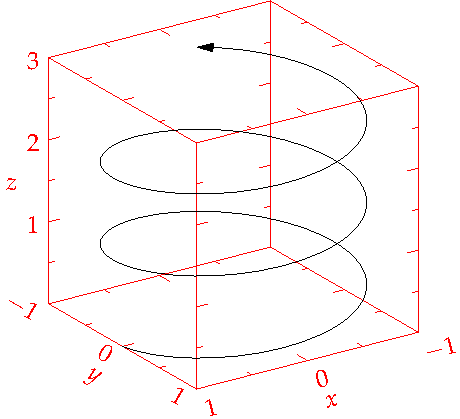
\includegraphics[width=\linewidth]{helix}
  \caption{This is a margin figure. The helix is defined by 
    $x = \cos(2\pi z)$, $y = \sin(2\pi z)$, and $z = [0, 2.7]$. The figure was
    drawn using Asymptote (\url{http://asymptote.sf.net/}).}
  \label{fig:marginfig}
\end{marginfigure}

\begin{Verbatim}
\begin{marginfigure}
  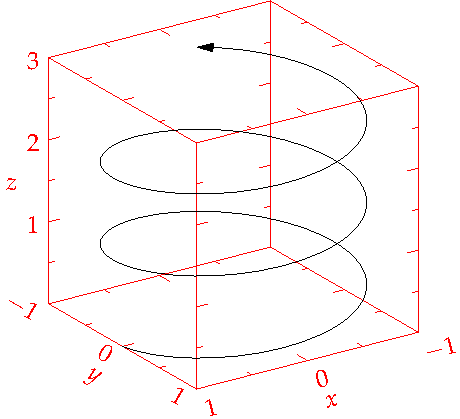
\includegraphics{helix}
  \caption{This is a margin figure.}
\end{marginfigure}
\end{Verbatim}

The \docenv{marginfigure} and \docenv{margintable} environments accept an
optional parameter \docopt{offset} that adjusts the vertical position of the
figure or table. See the ``\nameref{sec:sidenotes}'' section above for examples.
The specifications are:
\begin{docspec}
  \doccmd{begin\{marginfigure\}[\docopt{offset}]}\\
  \qquad\ldots\\
  \doccmd{end\{marginfigure\}}\\
  \mbox{}\\
  \doccmd{begin\{margintable\}[\docopt{offset}]}\\
  \qquad\ldots\\
  \doccmd{end\{margintable\}}\\
\end{docspec}

\Cref{fig:fullfig} is an example of the \Verb|figure*|
environment and \cref{fig:textfig} is an example of the normal
\Verb|figure| environment.

\begin{figure*}[h]
  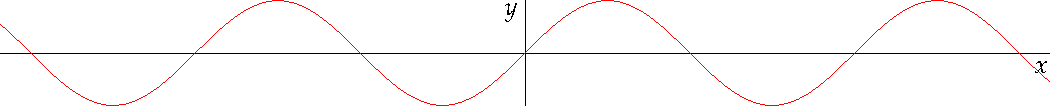
\includegraphics[width=\linewidth]{sine.pdf}%
  \caption{This graph shows $y = \sin x$ from about $x = [-10, 10]$.
  \emph{Notice that this figure takes up the full page width.}}%
  \label{fig:fullfig}%
\end{figure*}

\begin{figure}
  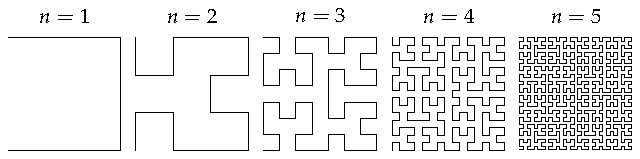
\includegraphics{hilbert-curves.pdf}
%  \checkparity This is an \pageparity\ page.%
  \caption{Hilbert curves of various degrees $n$.
  \emph{Notice that this figure only takes up the main textblock width.}}
  \label{fig:textfig}
  %\zsavepos{pos:textfig}
  \setfloatalignment{b}
\end{figure}

\Cref{tab:normaltab} shows table created with the \docpkg{booktabs}
package. Notice the lack of vertical rules---they serve only to clutter
the table's data.

\begin{table}[ht]
  \centering
  \fontfamily{ppl}\selectfont
  \begin{tabular}{ll}
    \toprule
    Margin & Length \\
    \midrule
    Paper width & \unit[8\nicefrac{1}{2}]{inches} \\
    Paper height & \unit[11]{inches} \\
    Textblock width & \unit[6\nicefrac{1}{2}]{inches} \\
    Textblock/sidenote gutter & \unit[\nicefrac{3}{8}]{inches} \\
    Sidenote width & \unit[2]{inches} \\
    \bottomrule
  \end{tabular}
  \caption{Here are the dimensions of the various margins used in the Tufte-handout class.}
  \label{tab:normaltab}
  %\zsavepos{pos:normaltab}
\end{table}

\section{Full-width text blocks}

In addition to the new float types, there is a \docenv{fullwidth}
environment that stretches across the main text block and the sidenotes
area.

\begin{Verbatim}
\begin{fullwidth}
Lorem ipsum dolor sit amet...
\end{fullwidth}
\end{Verbatim}

\begin{fullwidth}
\small\itshape\lipsum[1]
\end{fullwidth}

\section{Typography}\label{sec:typography}

\subsection{Typefaces}\label{sec:typefaces}
If you're using \hologo{XeLaTeX}\ or \hologo{LuaLaTeX}, the class will use ETbb as the main
typeface if the \texttt{etbb} package is installed and \TeX\ Gyre Pagella
otherwise; \textsf{\TeX\ Gyre Heros}, and \texttt{\TeX\ Gyre
Cursor} are the default for sans-serif and monospace text, respectively.
(The \TeX\ Gyre faces are usually included with \TeX\ Live
distributions.) In these cases, the class automatically loads the
\texttt{fontspec} package, so you can easily select your own system
fonts. Under pdf\LaTeX, the class defaults to the Palatino, \textsf{Helvetica},
and \texttt{Bera Mono} typefaces if they're installed. Otherwise,
we'll fall back on the Computer Modern typefaces.

\subsection{Letterspacing}\label{sec:letterspacing}
This document class includes two new commands and some improvements on
existing commands for letterspacing.

When setting strings of \allcaps{ALL CAPS} or \smallcaps{small caps}, the
letter\-spacing---that is, the spacing between the letters---should be
increased slightly.\cite{Bringhurst2005}  The \Verb|\allcaps| command has proper letterspacing for
strings of \allcaps{FULL CAPITAL LETTERS}, and the \Verb|\smallcaps| command
has letterspacing for \smallcaps{small capital letters}. These commands
will also automatically convert the case of the text to upper- or
lowercase, respectively.

The \Verb|\textsc| command has also been redefined to include
letterspacing. The case of the \Verb|\textsc| argument is left as is,
however. This allows one to use both uppercase and lowercase letters:
\textsc{The Initial Letters Of The Words In This Sentence Are Capitalized.}

\section{Installation}\label{sec:installation}
To install the Tufte-\LaTeX\ classes, simply drop the
following files into the same directory as your \texttt{.tex}
file:
\begin{quote}
  \ttfamily
  tufte-book.cls\\
  tufte-common.def\\
  tufte-handout.cls\\
  tufte.bst
\end{quote}

% TODO add instructions for installing it globally

\section{More Documentation}\label{sec:more-doc}
For more documentation on the Tufte-\LaTeX{} document classes (including commands not
mentioned in this handout), please see the sample book.

\section{Support}\label{sec:support}

The website for the Tufte-\LaTeX\ packages is located at
\url{https://github.com/Tufte-LaTeX/tufte-latex}. On our website, you'll find
links to our \smallcaps{svn} repository, mailing lists, bug tracker, and documentation.

% Print Bibliography
\printbibliography[heading=bibnumbered]

\end{document}
